%	현대물리실험 보고서
%	실험6 밀리칸 오일 실험
%	202100973 이승엽

%----------------------------------------------------------------------------------------
%	PACKAGES AND DOCUMENT CONFIGURATIONS
%----------------------------------------------------------------------------------------

\documentclass[a4paper, 10pt, nanum]{CSUniSchoolLabReport}
% use UTF8 encoding
\usepackage[utf8]{inputenc}
% use KoTeX package for Korean
\usepackage{kotex}
\usepackage{amsmath}
\usepackage{hyperref}
\usepackage{graphicx}
\usepackage{indentfirst}
\usepackage{setspace}
\usepackage{multirow}
\usepackage{enumitem}
\usepackage{graphicx}
\usepackage{wrapfig}

\setlength{\parindent}{0.2in} % 들여쓰기 길이 설정
\setlength{\parskip}{3mm} % 문단 간의 간격 조절
\setstretch{1.5} % 줄간격

\addbibresource{reference.bib} % Bibliography file (located in the same folder as the template)

%----------------------------------------------------------------------------------------
%	REPORT INFORMATION
%----------------------------------------------------------------------------------------

\title{현대물리실험 실험6 보고서 \\ Millikan's Oil Drop} % Report title

\author{\textsc{Department of Physics} 202100973 이승엽}

\date{\today}

%----------------------------------------------------------------------------------------

\begin{document}

\maketitle % Insert the title, author and date using the information specified above

\begin{center}
	\begin{tabular}{l r}
		Date Performed: & March 14, 2023 \\ % Date the experiment was performed
		Partners: & 202100969 이규리 \\ % Partner names
		& 202100989 한누리 \\
		Instructor: & Professor 이기주 % Instructor/supervisor
	\end{tabular}
\end{center}

%----------------------------------------------------------------------------------------
%	ABSTRACT
%----------------------------------------------------------------------------------------

\maketitle
% \begin{abstract}
% 	This report ...
% \end{abstract}

%----------------------------------------------------------------------------------------
%	INTRODUCTION
%----------------------------------------------------------------------------------------

\section{서론}

	입자의 전하량은 이미 알고 있는 세기의 전기장 하에서 입자가 받는 힘을 측정함으로써 계산할 수 있다. 특정한 값의 전기장을 만드는 것은 비교적 쉬운 일이지만, 겨우 한 개 또는 수 개의 과잉 전자만을 실어 나르는 입자에 작용하는 힘은 매우 작기 때문에 측정하기 힘들다. 

	밀리컨의 기름방울 실험은 이러한 작은 힘들을 얼마나 잘 측정할 수 있는지에 따라 성공 여부가 좌우된다. 

	이 실험을 통해 일차적으로 측정하는 것은 기름방울의 총 전하량이지만, 실험을 통해 얻은 데이터를 분석함으로써 단일 전자의 전하량을 결정할 수 있고 이를 위해서는 어느 정도 숙련된 실험 능력이 요구된다. 느리게 상승 및 하강하는 기름방울을 선택하면 적은 수의 과잉 전자를 포함하는 기름방울을 얻게 되는 것이다. 이러한 기름방울이 다수 관찰되어야 하며 이들 각각의 전하량이 계산되어야 한다. 이러한 기름방울의 전하량이 가장 작은 특정 전하량의 정수배인 경우, 전기의 원자적 특성을 잘 보여주는 것이다.(전하의 양자화) 그러나, 각 전하량을 측정하는데 서로 다른 기름방울이 사용되었기 때문에, 기름방울 자체가 전하량에 영향을 미치는 것이 아닌가 하는 질문이 여전히 제기될 수 있다. 이러한 불확실성은 특정 기름방울을 관찰하는 동안 기름방울의 전하량을 직접 변경해줌으로써 제거할 수 있다. 기름방울 근처에 위치한 이온화원을 이용하면 동일한 기름방울의 전하량을 여러 차례 변경할 수 있다. 동일한 기름방울에 대한 측정 결과가 가장 작은 특정 전하량의 정수배인 전하량을 산출한다면, 이는 전기의 원자적 특성에 대한 분명한 증거라 할 수 있다. 

%----------------------------------------------------------------------------------------
%	THEORY
%----------------------------------------------------------------------------------------

\section{이론}

	기름방울에 작용하는 힘들(중력, 전기력, 공기저항력)을 분석하면 기름방울의 전하량을 결정하는 수식을 얻을 수 있다.

\subsection{기름방울의 속도와 전기장 사이의 관계식 수립}

	기름방울이 공기 중에서 낙하할 때 및 종단 속도에 도달했을 때, 기름방울에 작용하는 힘을 나타내보자. (이 실험에서 사용되는 기름방울은 수 밀리세컨드 내에 종단 속도에 도달함.) 여기서 $v^2_f$는 종단 속력(terminal speed), $k$는 공기와 기름방울 사이의 마찰계수, $m$은 기름 방울의 질량, $g$는 중력가속도를 나타낸다. 마찰력 $F_f$와 중력 $F_g$는 크기가 같고 방향이 반대이므로, 다음과 같이 나타낼 수 있다.
	\begin{align*}
		\vec{F_f} + \vec{F_g} = 0
	\end{align*}
	\begin{align}
		\label{eqn:1}
		k = \frac{mg}{v_f}
	\end{align}

	전기장을 걸어주었을 때 상승하는 기름방울에 작용하는 힘을 보면, $E$는 전기장, $q$는 기름방울의 전하량이고, $v_r$은 상승 속도를 나타낸다. 받는 힘을 벡터적으로 더하면 다음과 같이 정리할 수 있다.
	\begin{align*}
		\vec{F_f} + \vec{F_g} + \vec{F_E} = 0
	\end{align*}
	\begin{align}
		\label{eqn:2}
		v_r = \frac{qv_f}{mg} E + v_f
	\end{align}

\subsection{질량 구하기}

	(Eq. \ref{eqn:2})로부터 질량 $m$을 구하기 위하여, 구의 부피에 대한 다음 식을 사용한다.
	\begin{align}
		\label{eqn:3}
		m = \frac{4}{3} \pi a^3 \rho
	\end{align}

	여기서 $a$는 기름방울의 반지름, $\rho$는 기름의 밀도이다.

	반지름 $a$를 계산하기 위하여, 점성 매질(점성계수가 $\eta$인) 내에서 구의 반지름과 낙하 속도와의 관계를 말해주는 스토크스 법칙(Stoke's Law)을 이용한다. 
	\begin{align}
		\label{eqn:4}
		a = \sqrt[]{\frac{9\eta v_f}{2g\rho}}
	\end{align}

	그러나 스토크스 법칙은 기름방울의 낙하 속도가 0.1 cm/s 이하일 경우 더 이상 정확하지 않다(상기 속도 이하의 속도를 갖는 기름방울은 공기 분자의 평균 자유 경로에 상응하는 2미크론 정도의 반지름을 가지므로, 이는 스토크스 법칙을 유도하면서 이루어진 가정 중 하나를 위반하게 됨). 이 실험에서 사용되는 기름방울의 속도는 0.05 $\sim$ 0.001 cm/s 이므로, 점성계수에 보정계수를 곱해야 한다. 이에 따른 유효 점성계수는 다음과 같다.
	\begin{align}
		\label{eqn:5}
		\eta_{eff} = \eta \frac{1}{1 + \frac{b}{pa}}
	\end{align}

	여기서 $b$는 상수(이 값은 (Eq. \ref{eqn:9}) 아래에 기재되어 있음), $p$는 대기압, $a$는 위의 보정되지 않은 스토크스 (Eq. \ref{eqn:4})에 의해 계산된 기름방울의 반지름이다. 
	(Eq. \ref{eqn:5})의 $\eta_{eff}$를 (Eq. \ref{eqn:4})에 대입하여, 반지름 $a$에 대해서 풀면 다음과 같다.
	\begin{align}
		\label{eqn:6}
		a = \sqrt{\left(\frac{b}{2p}\right)^2 + \frac{9\eta v_f}{2g\rho}} - \frac{b}{2p}
	\end{align}

	그러면 (Eq. \ref{eqn:3})을 이용해서 기름방울의 질량을 구할 수 있다.

\subsection{전하량 구하기}

	(Eq. \ref{eqn:2})를 살펴보면,
	\begin{align*}
		v_r = \frac{qv_f}{mg} E + v_f
	\end{align*}

	$v_r$대 $E$의 그래프로부터 다음과 같은 기울기 $s$를 얻을 수 있다.
	\begin{align}
		\label{eqn:7}
		s = \frac{qv_f}{mg}
	\end{align}

	이를 전하량 $q$에 관하여 정리하면 다음과 같다.
	\begin{align}
		\label{eqn:8}
		q = \frac{smg}{v_f}
	\end{align}

	위의 (Eq. \ref{eqn:3}) 및 (Eq. \ref{eqn:6})에서 구한 질량을 대입하면 전하량은 최종적으로 다음과 같다.
	\begin{align}
		\label{eqn:9}
		q = - \frac{\frac{4}{3}\pi gs\rho \left[ \sqrt{\left(\frac{b}{2p}\right)^2 + \frac{9\eta v_f}{2g\rho}} - \frac{b}{2p}\right]^3}{v_f}
	\end{align}

%----------------------------------------------------------------------------------------
%	EXPERIMENTAL METHOD
%----------------------------------------------------------------------------------------

\section{실험 방법}

\subsection{플랫폼의 높이 조절과 수평 맞추기}

\begin{enumerate}[label=\arabic*.]
	\item 실험자가 똑바로 앉아 기름방울을 관찰할 수 있는 높이에 관측경이 위치하도록, 일정 높이의 견고한 테이블 위에 장치를 놓는다. 적절한 높이에 도달하기 위해 필요하다면 장치를 큰 막대 스탠드	(ME-8735) 상의 두 개의 지지 막대(ME-8736) 위에 설치한다.
	\item 부착된 수평지시기(bubble level)를 사용하여 장치의 수평을 맞춘다. 이 때 막대 스탠드의 수평조절 나사(leveling Screws) 또는 플랫폼의 수평 조절 발(leveling feet)을 이용하면 된다.
	
	\begin{figure}[htb!]
		\centering
		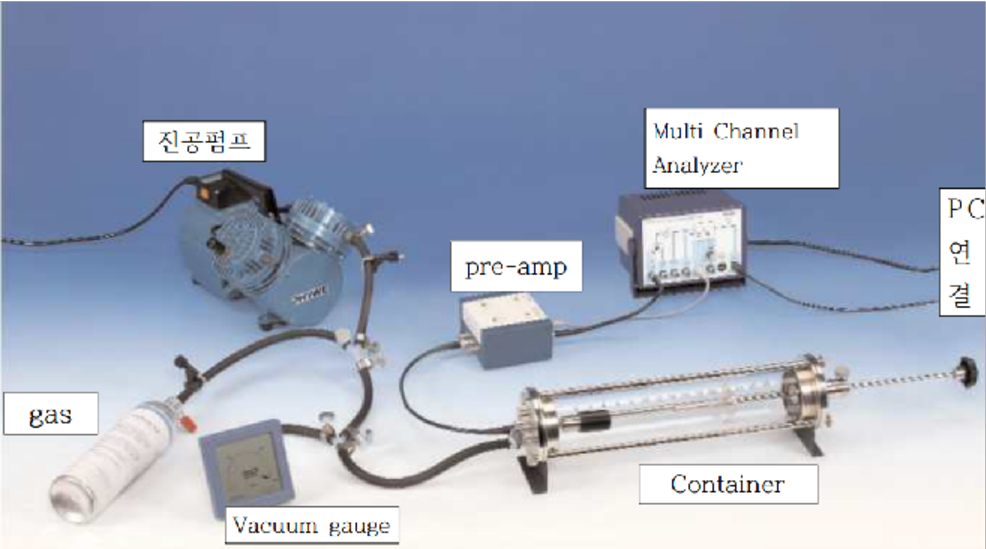
\includegraphics[width=5cm]{fig1.eps}
		\caption{}
		\label{fig:1}
	\end{figure}
\end{enumerate}

\subsection{실험실 셋팅 조절}

\begin{enumerate}[label=\arabic*.]
	\item 실험실 조명을 가능한 한 어둡게 하되, 멀티미터 및 스톱워치를 읽거나 데이터를 기록할 수 있을 정도로 빛의 양을 조절한다.
	\item 장치 뒤의 배경이 어두워야 한다.
	\item 통풍 및 진동이 없는 위치를 선택한다.
\end{enumerate}

\subsection{플레이트 간격 측정}

\begin{enumerate}[label=\arabic*.]
	\item 하우징(회색 원기둥)을 똑바로 들어올리고, 상부 캐패시터 플레이트(금색) 및 스페이서 플레이트(투명)를 제거하여 기름방울 관측 챔버를 분해한다. 하우징에 삽입되어 있는 스펀지를 제거한다.

	\begin{figure}[htb!]
		\centering
		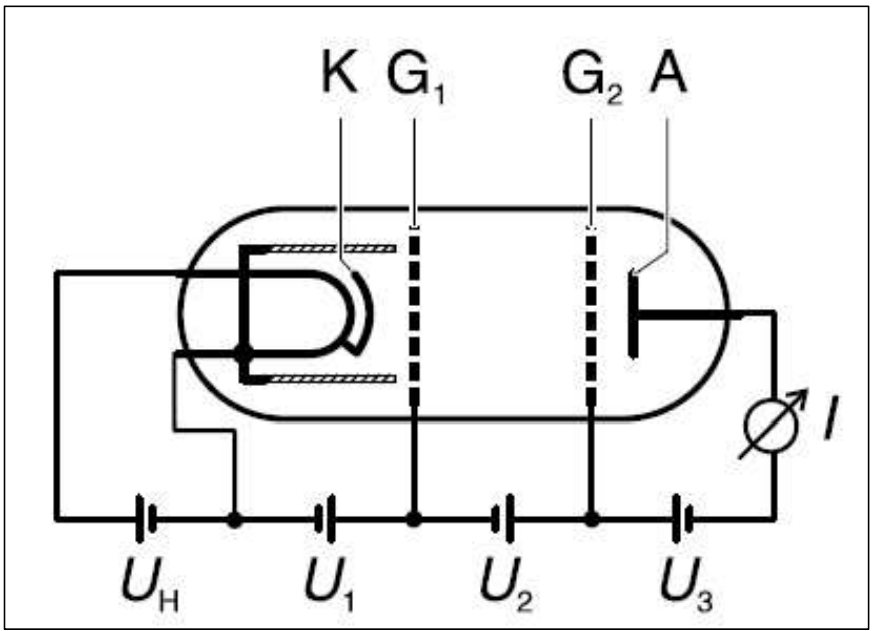
\includegraphics[width=5cm]{fig2.eps}
		\caption{}
		\label{fig:2}
	\end{figure}

	\item 마이크로미터로 플라스틱 스페이서의 두께(플레이트 사이의 거리와 동일함)를 측정한다. 스페이서의 튀어나온 테두리가 측정치에 포함되지 않도록 주의한다. 이 측정치의 	정확성은 실험 결과의 정확도에 중요한 영향을 미친다. 측정치를 기록한다.

	\begin{figure}[htb!]
		\centering
		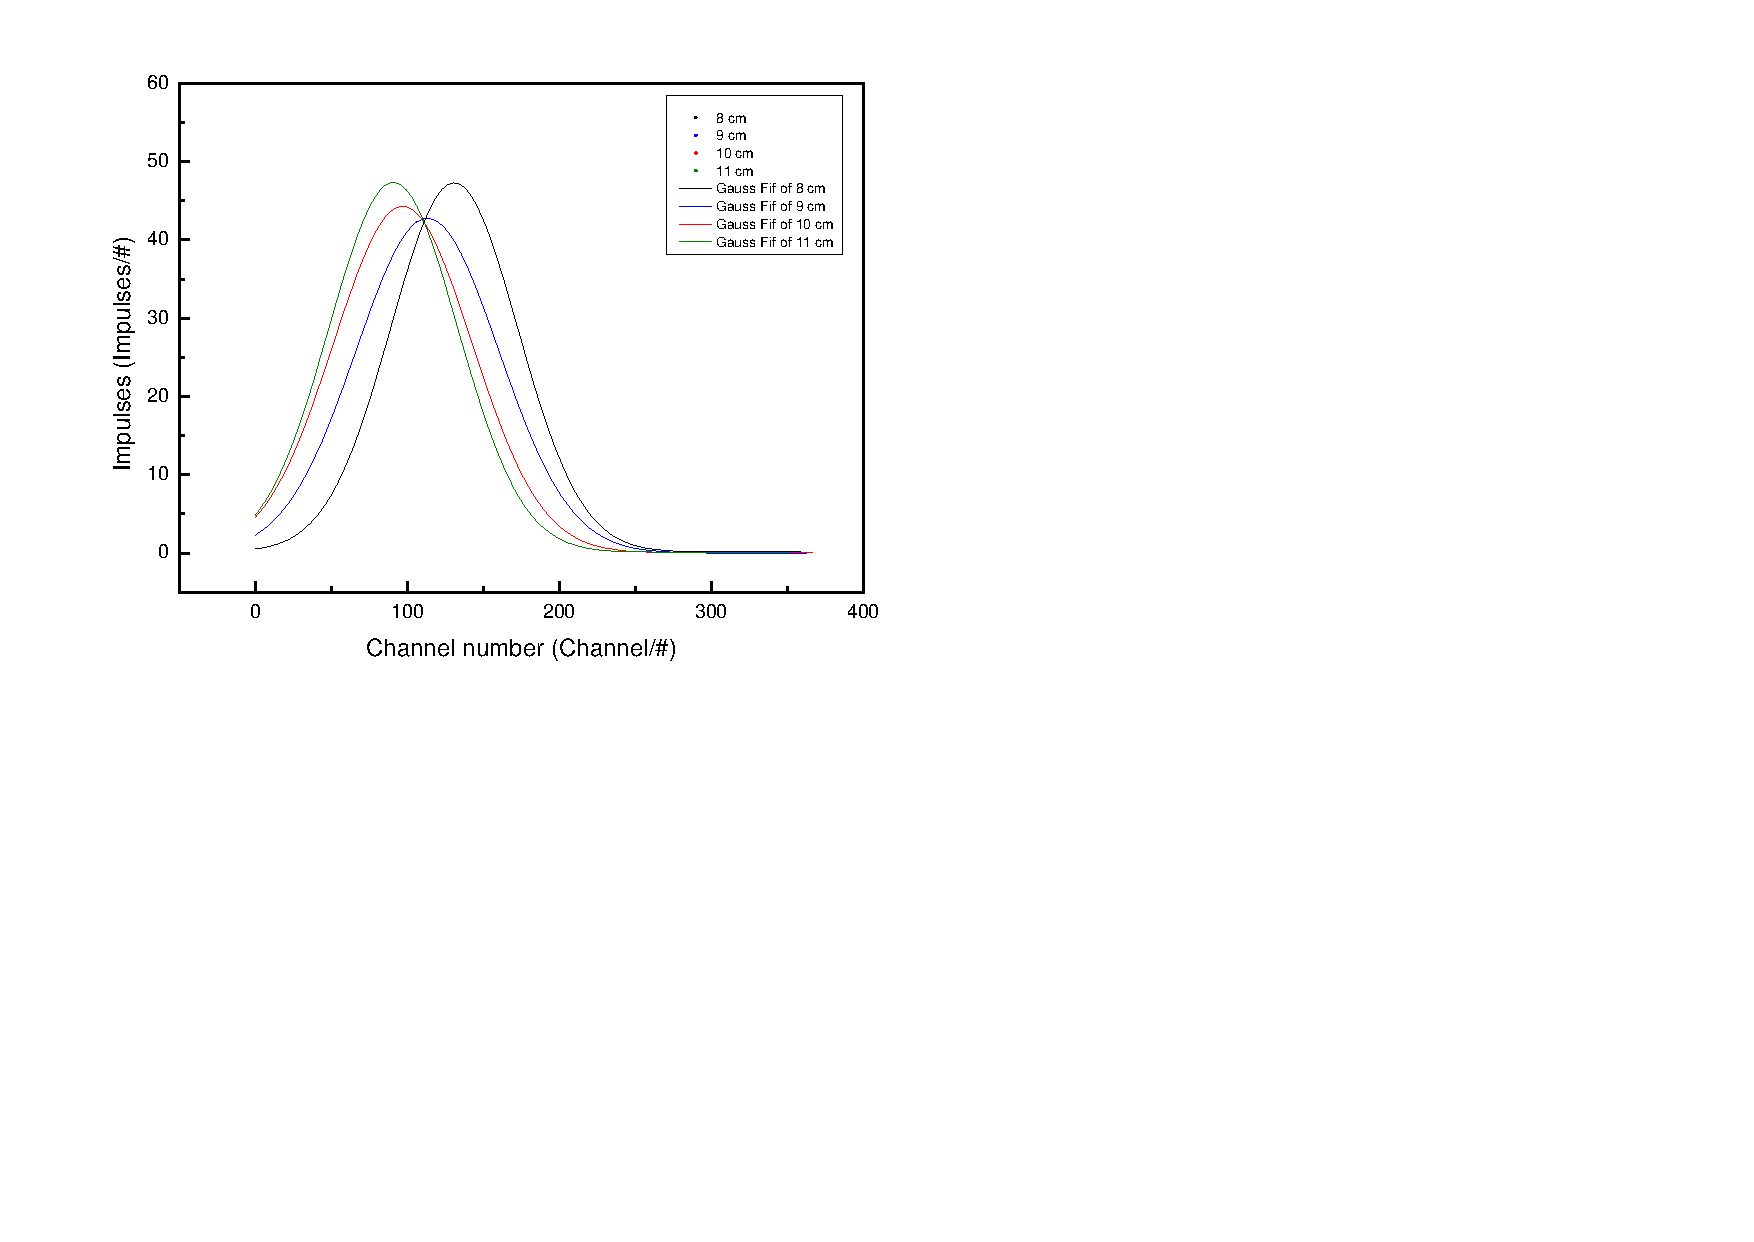
\includegraphics[width=5cm]{fig3.eps}
		\caption{}
		\label{fig:3}
	\end{figure}

\end{enumerate}

\subsection{광학 시스템 정렬}

\subsubsection{관측경의 초점 맞추기}

\begin{enumerate}[label=\arabic*.]
	\item 하부 캐패시터 플레이트(금색) 위에 플라스틱 스페이서와 상부 캐패시터 플레이트를 재조립한다. 하우징 핀을 이용해 베이스의 구멍을 정렬시키면서 하우징의 위치를 다시 잡는다.
	\item 플랫폼에서 포커싱 와이어를 분리하여, 이를 상부 캐패시터 플레이트의 중앙에 위치한 구멍에 조심스럽게 삽입한다.
	\item 12 V DC 변압기를 할로겐 램프 하우징에 있는 램프 전원 잭에 연결하고, 플러그를 벽면의 콘센트에 꽂는다. 변압기가 올바른 전압(100, 117, 220 또는 240 V)인지 확인한다
	\item 십자망 포커싱 링을 돌려 십자망에 초점을 맞춘다.
	\item 관측경을 통해 포커싱 와이어를 보면서, 포커싱 링을 돌려 와이어가 선명하게 보이도록 초점을 맞춘다.
\end{enumerate}

\subsubsection{할로겐 필라멘트의 초점 맞추기}

\begin{enumerate}[label=\arabic*.]
	\item 수평 필라멘트 조절 손잡이를 조절한다. 와이어의 우측 가장자리가 가장 밝은 경우 (와이어의 중앙에 비해 최고의 명암대비로) 빛의 초점이 가장 잘 맞춰진 것이다.
	\item 관측경을 통해 포커싱 와이어를 관찰하면서 빛이 십자망의 영역 중에 와이어 상에서 가장 밝을 때까지 수직 필라멘트 조절 노브를 돌린다.
	\item 포커싱 와이어를 플랫폼 상의 축전 위치로 되돌려 놓는다.
\end{enumerate}	

\subsection{전압의 조절 및 측정}

\begin{enumerate}[label=\arabic*.]
	\item 바나나 플러그 패치 코드를 이용하여, 고전압 DC 전원 공급 장치를 플레이트 전압 커넥터에 연결하고 약 500 V를 전달하도록 조절한다.
	
	\begin{figure}[htb!]
		\centering
		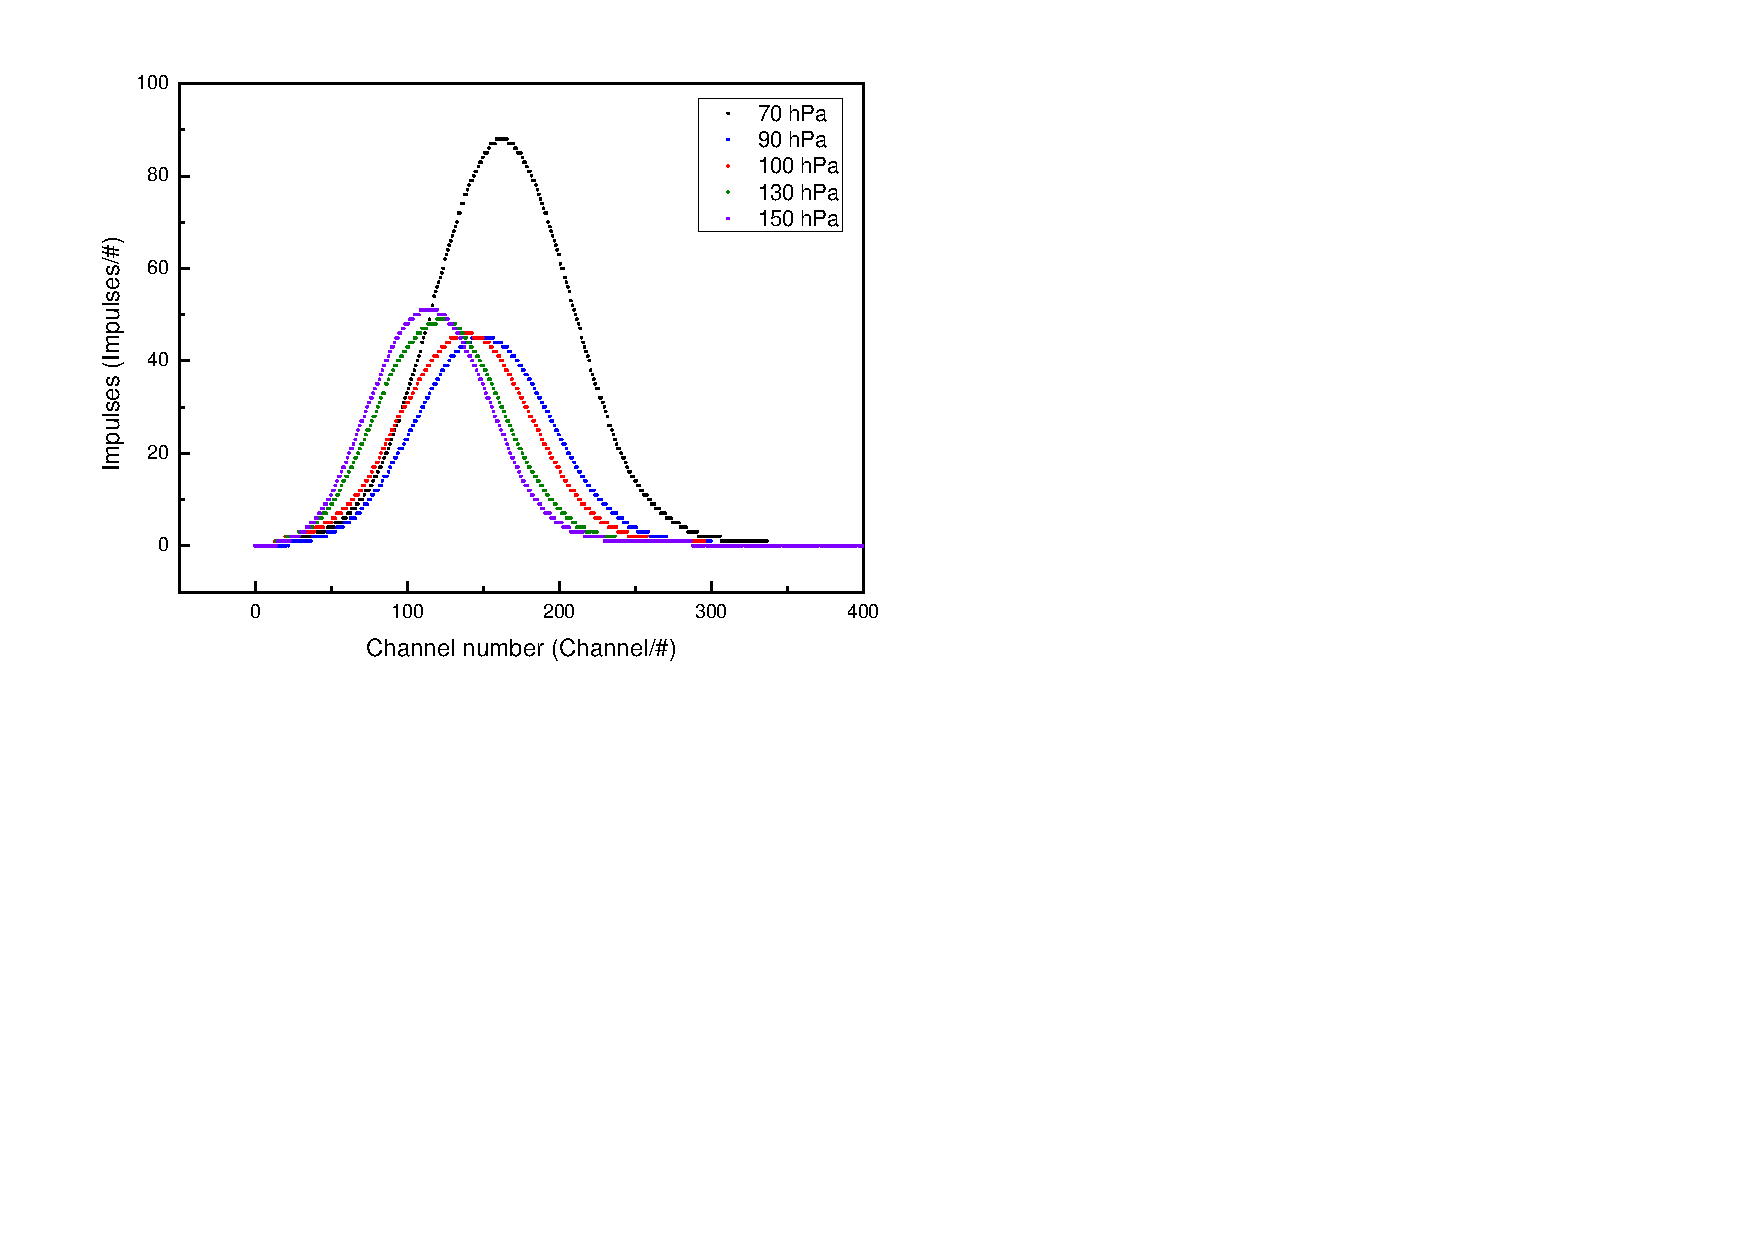
\includegraphics[width=5cm]{fig4.eps}
		\caption{}
		\label{fig:4}
	\end{figure}

	\item 디지털 멀티미터를 이용하여 상단 캐패시터 플레이트에 전달되는 전압을 측정한다. 캐패시터 플레이트 양단에 걸리는 전압이 아니라, 플레이트 전압 커넥터 (전원 공급 장치와 연결된 플러그 부분)에서의 전압을 측정한다. 전기 쇼크를 방지하기 위해 10 M$\Omega$ 저항기가 각 플레이트에 직렬로 연결되어 있다.
	
	\begin{figure}[htb!]
		\centering
		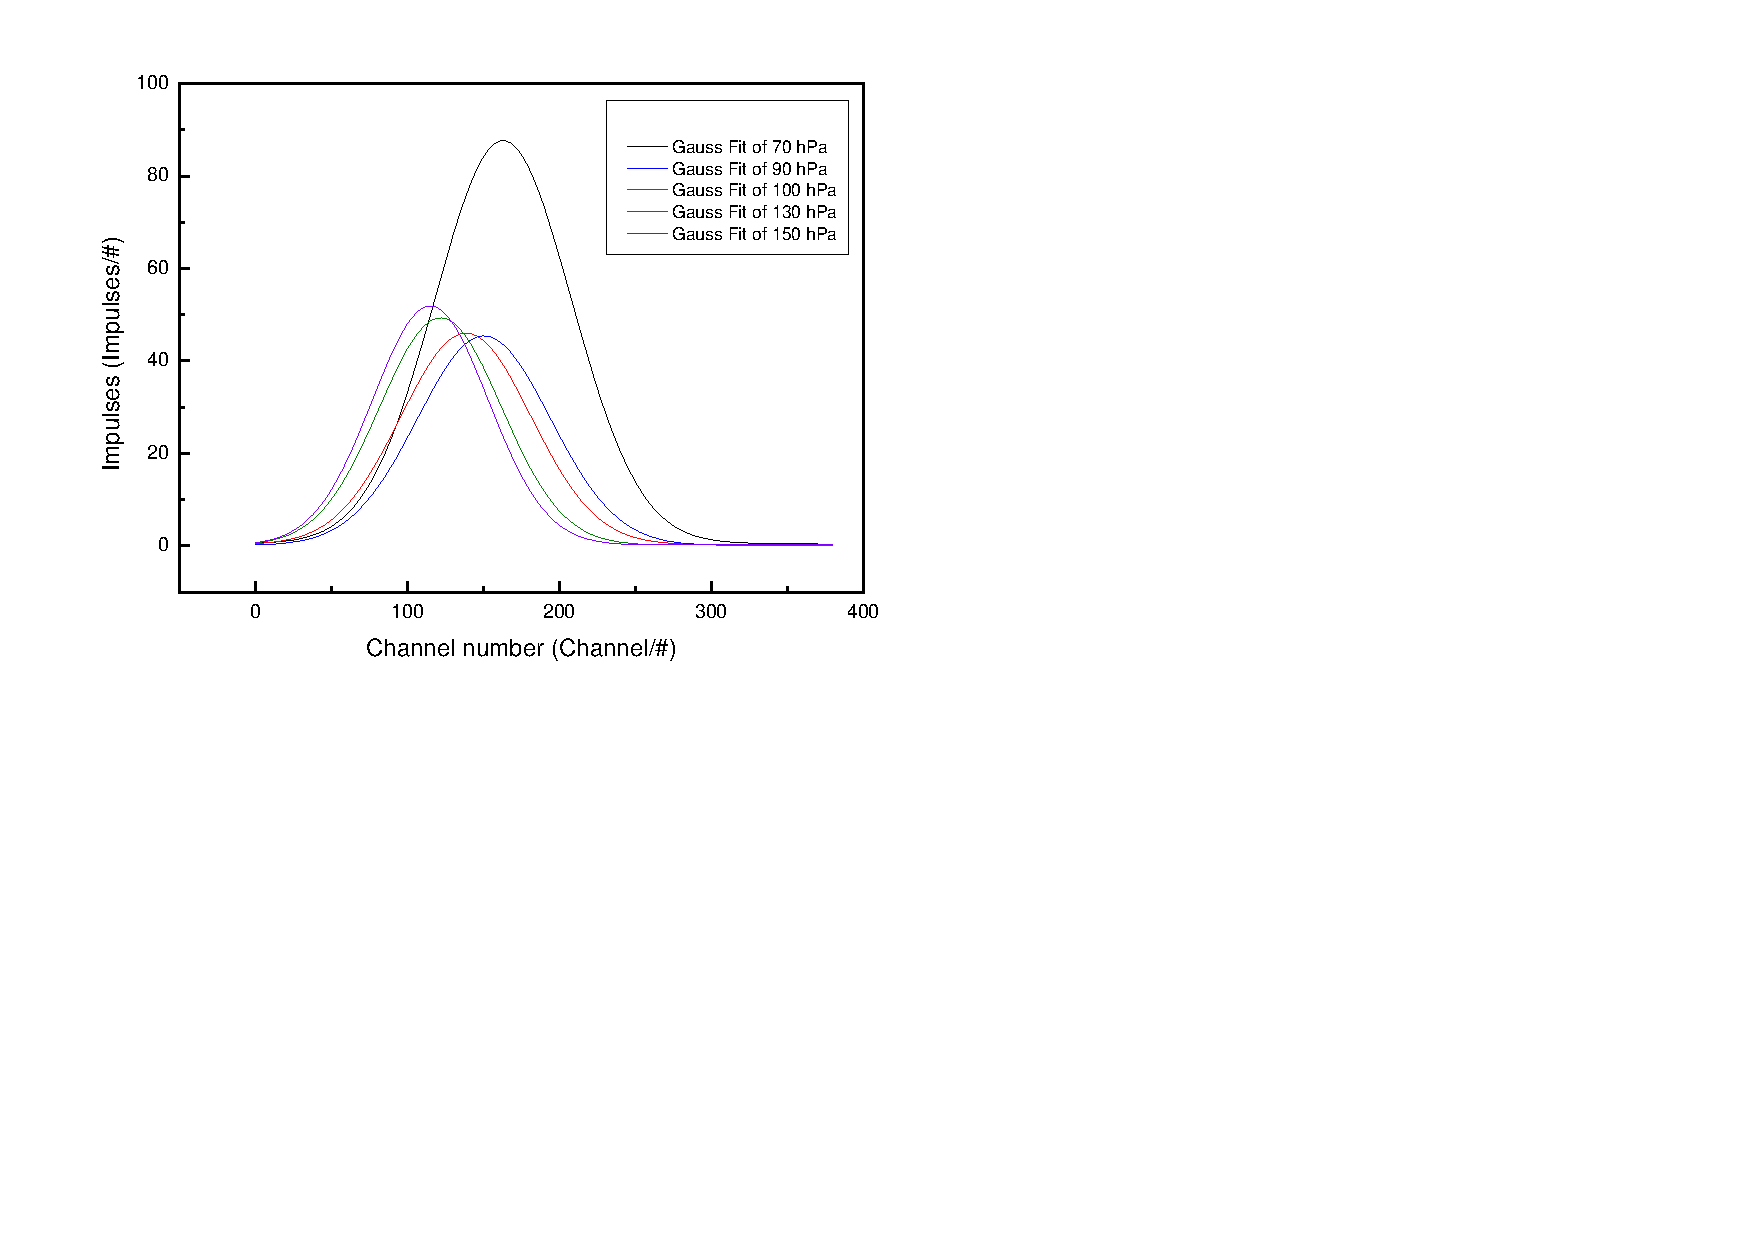
\includegraphics[width=5cm]{fig5.eps}
		\caption{}
		\label{fig:5}
	\end{figure}

\end{enumerate}

\subsection{기름방울 관측 챔버의 온도 측정}

\begin{enumerate}[label=\arabic*.]
	\item 멀티미터를 서미스터 커넥터에 연결하여 서미스터의 저항을 측정한다. 플랫폼에 위치한 서미스터 저항 표를 참조하여 하부 놋쇠(brass) 플레이트의 온도를 구한다. 측정된 온도는 기름방울 관측 챔버 내의 온도와 일치해야 한다.
	
	\begin{figure}[htb!]
		\centering
		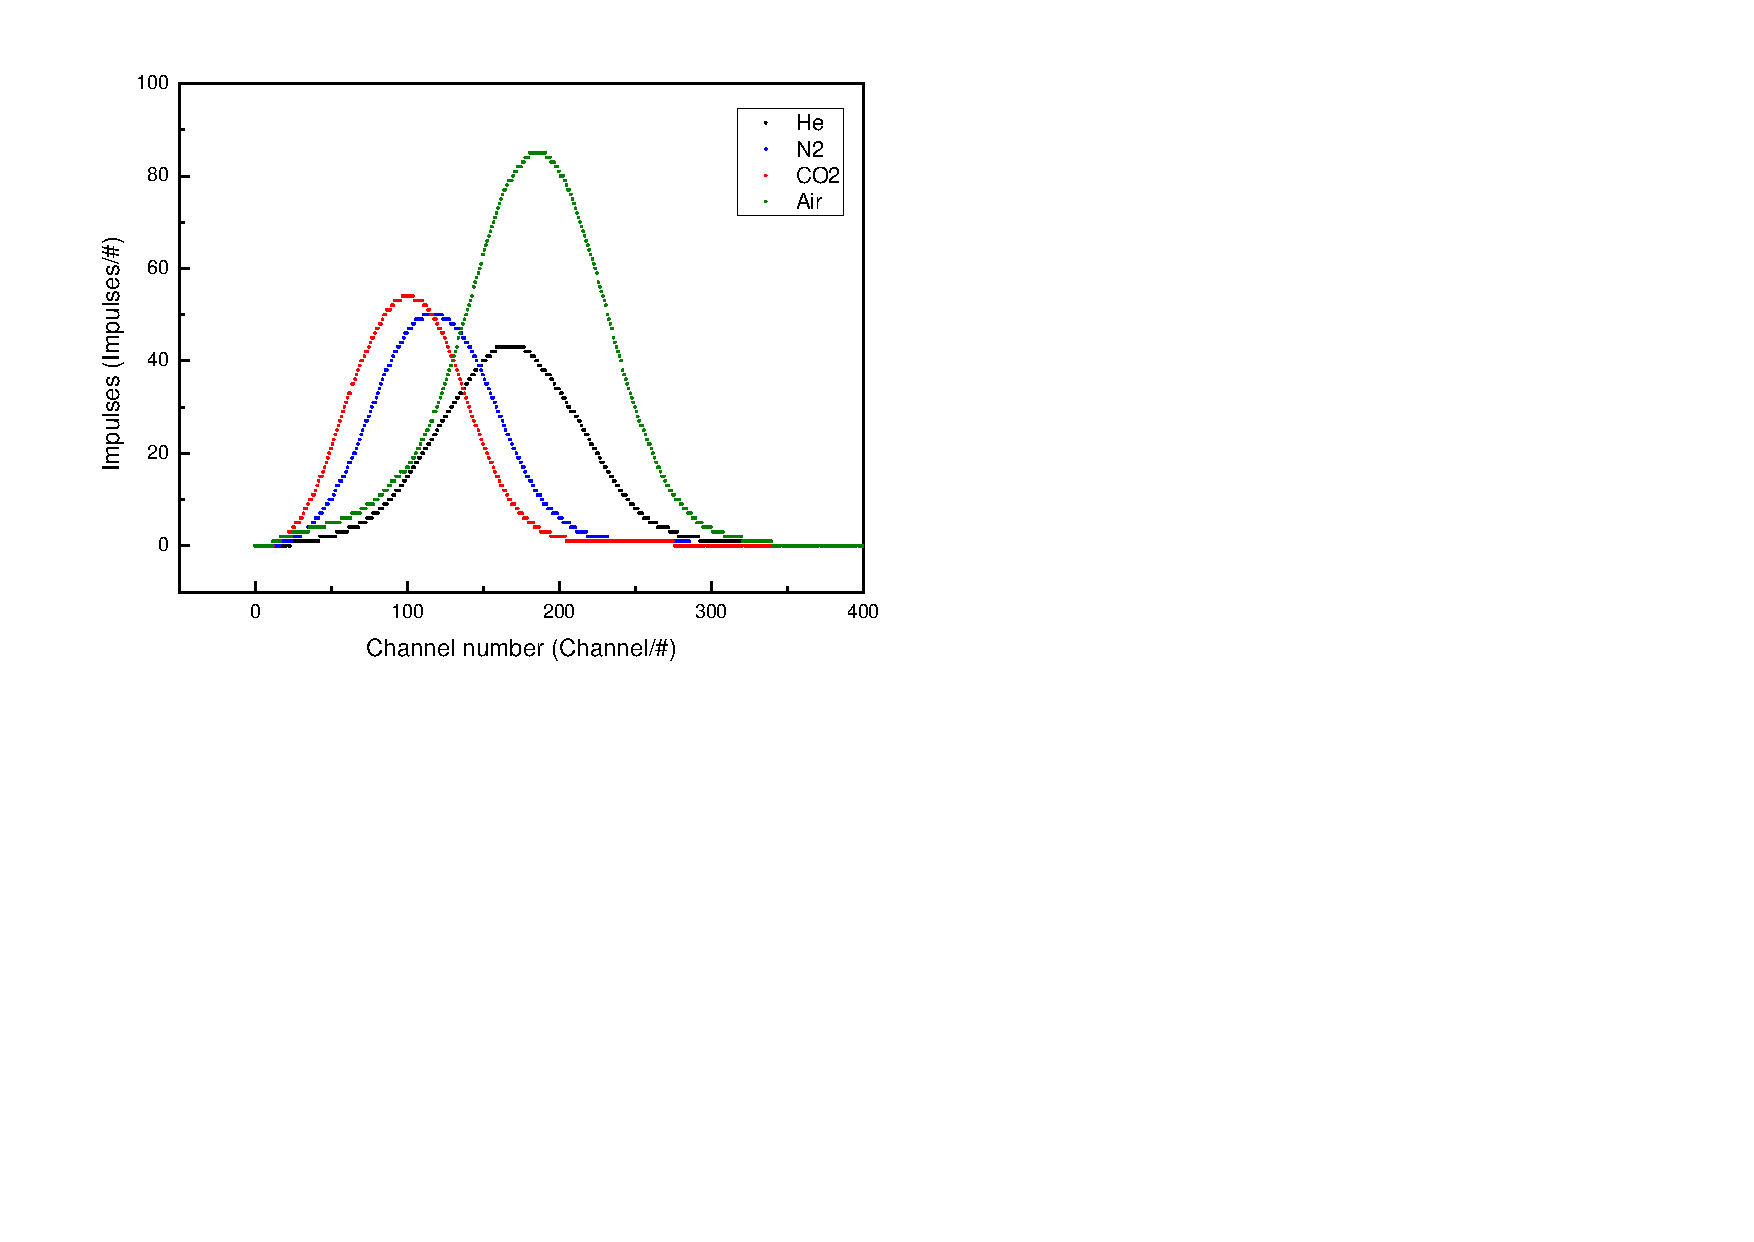
\includegraphics[width=5cm]{fig6.eps}
		\caption{}
		\label{fig:6}
	\end{figure}

	색선별(dichroic) 창은 할로겐 램프에 의해 생성된 열의 대부분을 반사하지만, 기름방울 관측 챔버 내의 온도는 빛에 장기간 노출된 후 상승하게 된다. 따라서 기름방울 관측 챔버 내의 온도는 주기적으로 측정해야 한다. (약 15분마다)

	\begin{figure}[htb!]
		\centering
		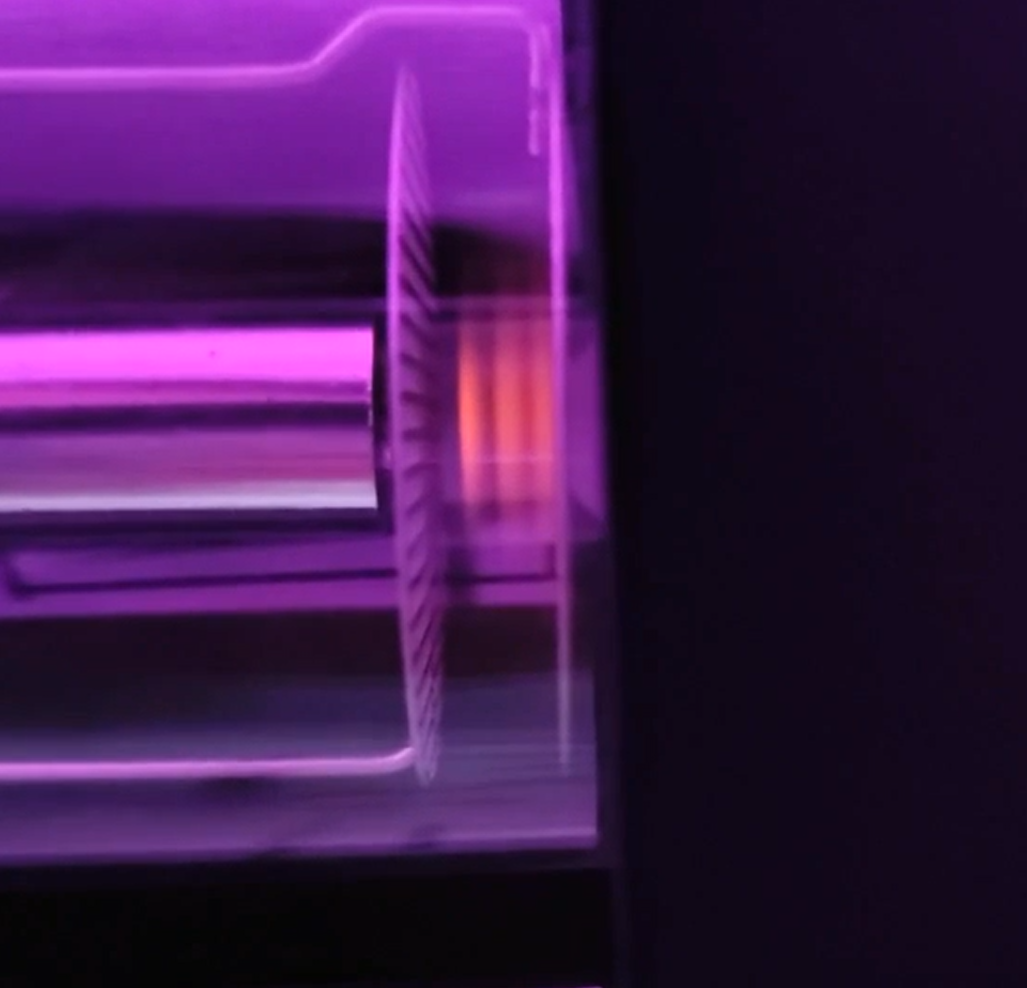
\includegraphics[width=5cm]{fig7.eps}
		\caption{}
		\label{fig:7}
	\end{figure}

	\begin{figure}[htb!]
		\centering
		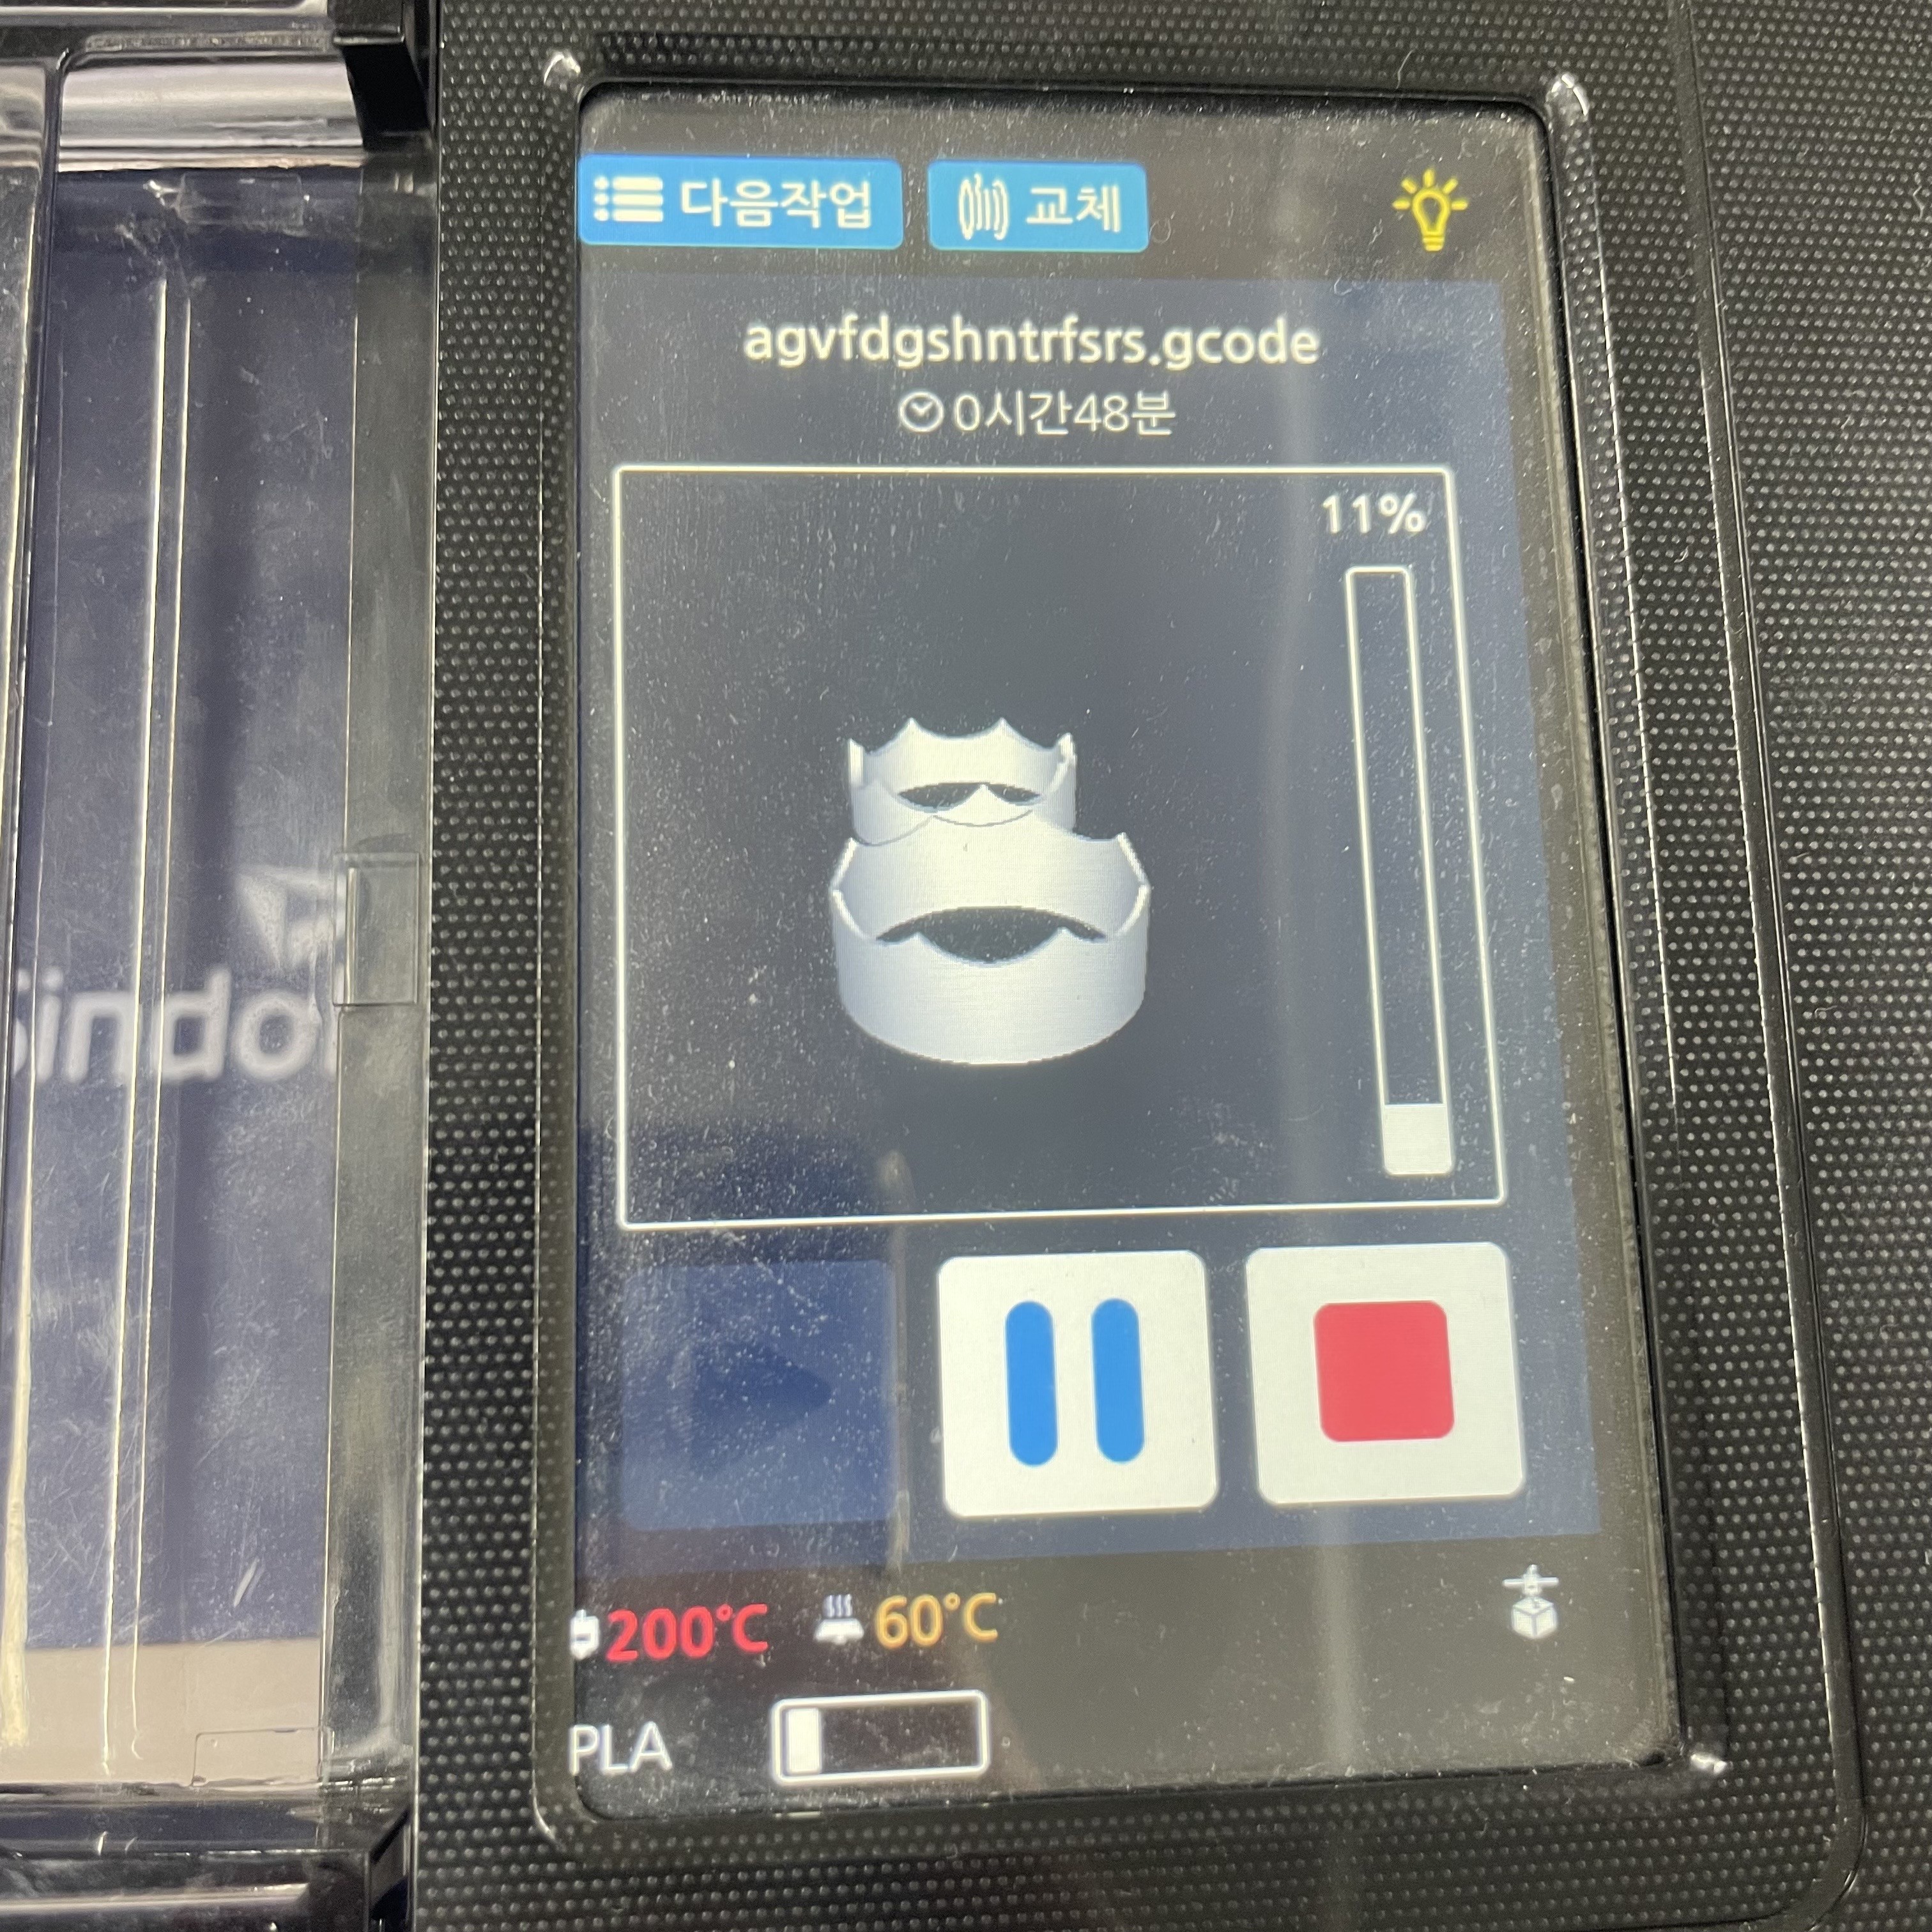
\includegraphics[width=5cm]{fig8.eps}
		\caption{}
		\label{fig:8}
	\end{figure}

	\begin{figure}[htb!]
		\centering
		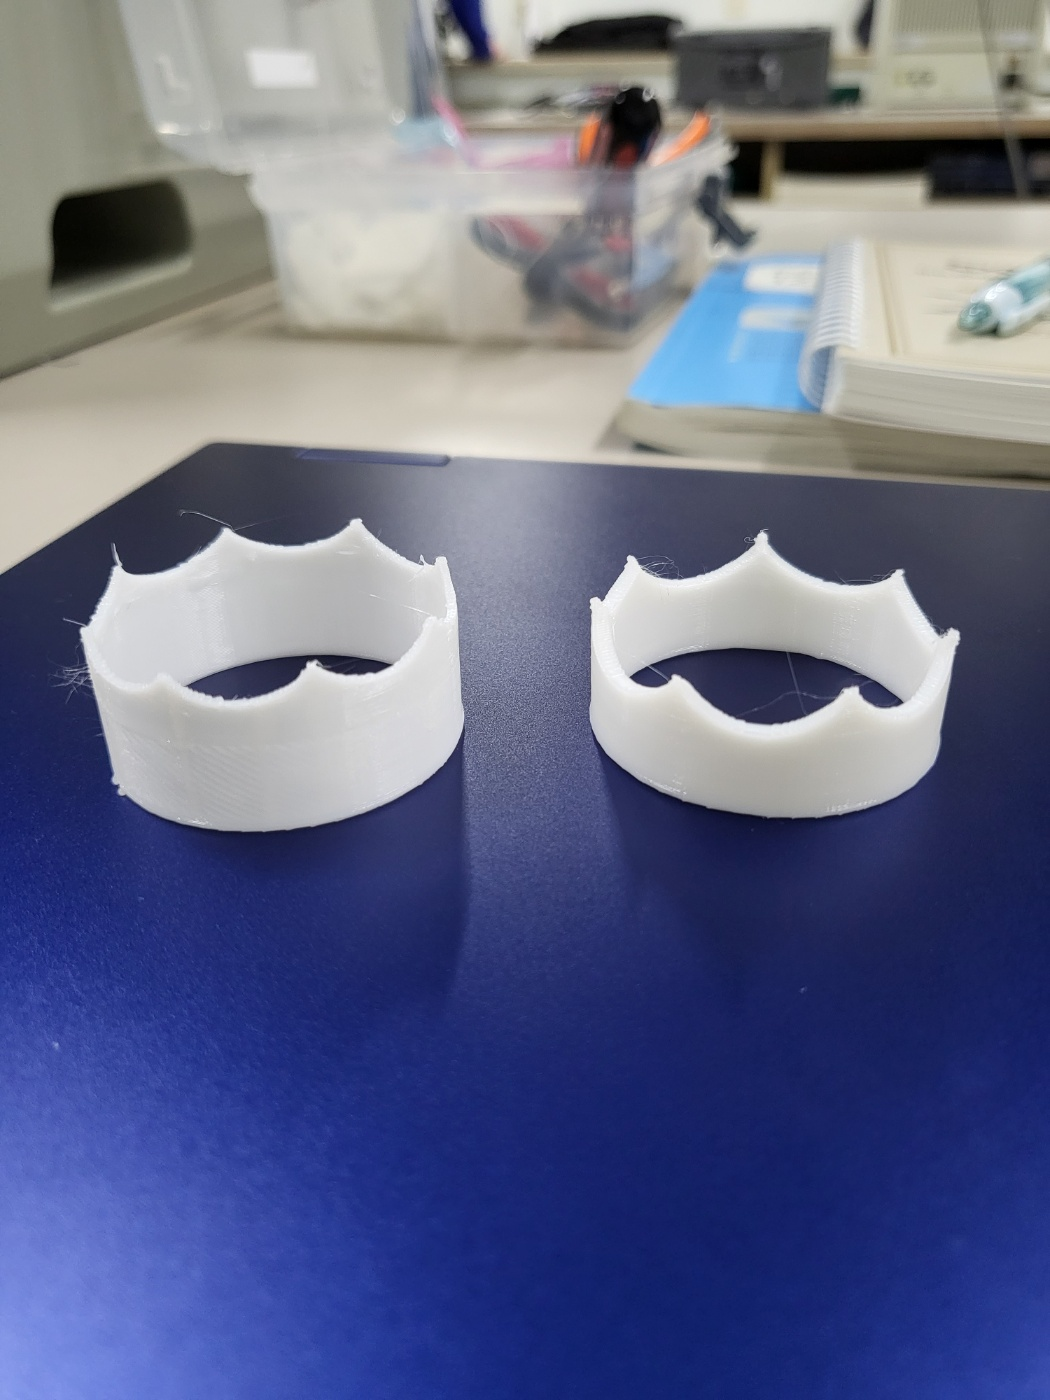
\includegraphics[width=5cm]{fig9.eps}
		\caption{}
		\label{fig:9}
	\end{figure}

\end{enumerate}

\subsection{}

\begin{enumerate}[label=\arabic*.]
	\item 상부 캐패시터 플레이트 위에 기름방울 구멍 덮개를 올려놓고 하우징 뚜껑을 덮어 기름방울 관측 챔버의 재조립을 완료한다.
	\item 플레이트 전압 및 서미스터 저항(온도)을 측정 및 기록한다.
	
	\begin{figure}[htb!]
		\centering
		\includegraphics[width=5cm]{fig10.eps}
		\caption{}
		\label{fig:10}
	\end{figure}

\end{enumerate}

\subsection{챔버 내로 기름방울 유입시키기}

\begin{enumerate}[label=\arabic*.]
	\item 이미 알려진 밀도의 비휘발성 기름을 분무기에 넣는다.
	\item 기름이 분사될 때까지 벌브를 빠르게 압착하여 분무기를 준비한다. 분무기의 끝부분의 뚜껑을 제거한 후 분사 부분을 아래쪽을 꺾어준 후 사용한다.
	\item 기름방울을 챔버 내로 유입시키는 동안 공기가 챔버에서 빠져 나갈 수 있도록 이온화 소스 레버를 방울 분사 위치(Spray Droplets Position)로 이동시킨다.
	\item 분무기의 노즐을 방울 관측 챔버 뚜껑 위의 구멍에 위치시킨다.
	\item 관측경을 통해 관찰하면서, 분무기 벌브를 한 번에 빠르게 압착시킨다. 그리고 벌브를 느리게 압착시켜, 기름방울 구멍 덮개의 구멍과 상부 캐패시터 플레이트의 기름방울 유입구멍을 통해 두 개의 캐패시터 플레이트 사이의 공간으로 기름방울을 밀어 넣는다.
	\item 관측경을 통해 기름방울의 낙하가 관찰되면 이온화 소스 레버를 OFF 위치로 이동시킨다.
	
	\begin{figure}[htb!]
		\centering
		\includegraphics[width=5cm]{fig11.eps}
		\caption{}
		\label{fig:11}
	\end{figure}

	\begin{figure}[htb!]
		\centering
		\includegraphics[width=5cm]{fig12.eps}
		\caption{}
		\label{fig:12}
	\end{figure}

\end{enumerate}

\subsection{기름방울의 선택}

\begin{enumerate}[label=\arabic*.]
	\item 관측 영역내의 기름방울 중에서, 플레이트 충전 스위치가 “플레이트 접지(Plates Grounded)” 위치에 있을 때 느리게(약 0.02–0.05 mm/s) 낙하하는 것, 그리고 전압을 가했을 때 상하로 움직여 주는 기름	방울을 선택한다. 너무 밝지 않은 기름방울을 선택한다. 극성을 변경할 때 너무 급작스럽게 반응하지 않는 기름방울을 선택한다.
	
	\begin{figure}[htb!]
		\centering
		\includegraphics[width=5cm]{fig13.eps}
		\caption{}
		\label{fig:13}
	\end{figure}

	\item 적당한 크기와 전하량을 가지는 기름방울을 발견한 경우, 관측경의 초점을 정밀하게 조절한다.  
\end{enumerate}

\subsection{데이터 수집}

	두 명이 함께 데이터를 수집할 것을 제안한다. 한 명은 한 손으로 플레이트 전압을 변화시키고 다른 손으로 스톱워치를 조작하면서 기름방울을 관찰한다. 또 한 명은 스톱워치를 읽고, 전압을 변화시키고, 데이터를 기록한다. 

\begin{enumerate}[label=\arabic*.]
	\item 기름방울이 관측 영역의 상단으로 “이끌리도록” 플레이트 전압을 변화시킨다. 
	\item 플레이트 전압을 “중립”으로 설정하고 기름방울이 1.00 mm의 거리 또는 2개의 큰 눈금 거리를 낙하할 때의 시간을 측정한다. 종단 속도 $v_f$에 대한 평균을 구하기 위해 이 과정을 수차례 반복한다.
	\item 전압을 500 V로 조정한다. 동일한 기름방울을 관측 영역의 상부로 이동시킨다. 기름방울이 아래로 움직이도록 플레이트 전압을 설정한다. 기름방울이 아래로 움직이는데 필요한 전압 및 극성을 기록한	다. ( -500 V 또는 +500 V)
	\item 기름방울이 1.0 mm의 거리 또는 2개의 큰 눈금 거리를 아래로 이동하는데 걸리는 시간을 구한다. 데이터 표에 이 값을 기록한다. (아래 방향으로 움직이는 것을 (-)로 함)
	\item 기름방울이 위로 움직이도록 플레이트 전압을 변화시킨다. 기름방울을 위로 이동시키는데 필요한 전압 및 극성을 기록한다.
	\item 기름방울이 1.0 mm의 거리 또는 2개의 큰 눈금 거리를 위로 이동하는데 걸리는 시간을 구한다. 데이터 표에 이 값을 기록한다.
	\item 400 V, 300 V, 200 V 및 100 V의 전압 값을 이용하여 3 $\sim$ 6 단계를 반복한다.

\end{enumerate}

%----------------------------------------------------------------------------------------
%	RESULT AND DISCUSSION
%----------------------------------------------------------------------------------------

\section{실험 결과 및 해석}

%----------------------------------------------------------------------------------------
%	EXPERIMENTAL DATA AND ANALYSIS
%----------------------------------------------------------------------------------------

\subsection{실험 데이터 및 분석}

스페이서 두께 $d$는 9.00 mm이며, 저항값을 통해 온도가 섭씨 15도임을 알 수 있다. 이를 통해 계산하면 다음과 같다.

\begin{table}[htb!]
	\label{tab:1}
	\centering
	\caption{이온화 오일의 전압에 따른 종단 및 상승, 하강 시간에 관한 표이다.}
	\begin{tabular}{c|c|ccc}
		\noalign{\smallskip}\noalign{\smallskip}\hline\hline
		\multirow{2}{*}{Voltage (V)} & \multirow{2}{*}{이동거리 (mm)} & \multicolumn{3}{c}{Time (s)} \\
		\cline{3-5}
			  &  & Terminal & 상승 & 하강 \\
		\hline
	 		500 & 10.0 & 41.39 & 28.09 & 11.97 \\
	 		400 & 5.0  & 9.70  & 8.24  & 3.02  \\
	 		300 & 5.0  & 9.70  & 12.15 & 3.81  \\
			200 & 5.0  & 17.22 & 5.31  & 3.34  \\
			100 & 5.0  & 28.72 & 12.95 & 7.67  \\
		\hline
		\hline
	\end{tabular}
\end{table}



\begin{table}[htb!]
	\label{tab:2}
	\centering
	\caption{이온화 오일의 전압에 따른 종단 및 상승, 하강 속도에 관한 표이다. $v_f$는 종단속도이며, $v_r$은 상승속도, $v_d$는 하강속도이다.}
	\begin{tabular}{c|cccc}
		\noalign{\smallskip}\noalign{\smallskip}\hline\hline
		\multirow{2}{*}{Voltage (V)} & \multicolumn{4}{c}{Velocity (m/s)} \\
		\cline{2-5}
			  & $v_{f1}$ & $v_{f2}$ & $v_r$ & $v_d$ \\
		\hline
	 		500 & $2.53\times 10^{-4}$ & $2.31\times 10^{-4}$ & $3.56\times 10^{-4}$ & $8.35\times 10^{-4}$  \\
	 		400 & $5.10\times 10^{-4}$ & $7.49\times 10^{-4}$ & $6.07\times 10^{-4}$ & $16.56\times 10^{-4}$ \\
	 		300 & $5.10\times 10^{-4}$ & $7.49\times 10^{-4}$ & $4.12\times 10^{-4}$ & $13.12\times 10^{-4}$ \\
			200 & $2.87\times 10^{-4}$ & $2.94\times 10^{-4}$ & $9.42\times 10^{-4}$ & $14.97\times 10^{-4}$ \\
			100 & $1.62\times 10^{-4}$ & $1.88\times 10^{-4}$ & $3.86\times 10^{-4}$ & $6.52\times 10^{-4}$  \\
		\hline
		\hline
	\end{tabular}
\end{table}


\begin{figure}[htb!]
	\centering
	\includegraphics[viewport=1mm 99mm 180mm 200mm, width=9cm, clip=true]{data_graph.eps}
	\caption{오일의 전하량에 대한 오일의 전하량($q$)과 전자의 전하량의 비($q/e$)이다.}
	\label{fig:exam}
\end{figure}

데이터가 오일의 전하량과 전자의 전하량의 비의 정부배 부분에 모여있음을 알 수 있다.

%----------------------------------------------------------------------------------------
%	CONCLUSIONS
%----------------------------------------------------------------------------------------

\section{결론}

밀리칸 오일 실험으로 오일의 전하량이 전자의 전하량의 정부배임을 알 수 있다. 이를 통해 전기의 원자적 특성에 대한 분명한 증거가 될 수 있음을 알 수 있다.

실험 데이터가 부족하여 오차 및 정확도를 구할 수 없었으나, 데이터가 많았다면 정수배 부분이 peak인 Gaussian function의 형태로 나타났을 것으로 본다.

%----------------------------------------------------------------------------------------
%	BIBLIOGRAPHY
%----------------------------------------------------------------------------------------

\printbibliography % Output the bibliography

%----------------------------------------------------------------------------------------

\end{document}